% ****** Start of file aipsamp.tex ******
%
%   This file is part of the AIP files in the AIP distribution for REVTeX 4.
%   Version 4.1 of REVTeX, October 2009
%
%   Copyright (c) 2009 American Institute of Physics.
%
%   See the AIP README file for restrictions and more information.
%
% TeX'ing this file requires that you have AMS-LaTeX 2.0 installed
% as well as the rest of the prerequisites for REVTeX 4.1
%
% It also requires running BibTeX. The commands are as follows:
%
%  1)  latex  aipsamp
%  2)  bibtex aipsamp
%  3)  latex  aipsamp
%  4)  latex  aipsamp
%
% Use this file as a source of example code for your aip document.
% Use the file aiptemplate.tex as a template for your document.
\documentclass[%
 aip,
 jmp,%
 amsmath,amssymb,
%preprint,%
 reprint,%
%author-year,%
%author-numerical,%
]{revtex4-1}

\usepackage{graphicx}% Include figure files
\usepackage{dcolumn}% Align table columns on decimal point
\usepackage{bm}% bold math
%\usepackage[mathlines]{lineno}% Enable numbering of text and display math
%\linenumbers\relax % Commence numbering lines
\usepackage{amsmath}
\usepackage{tikz}
\usepackage{adjustbox}
\usepackage{color}



\newcommand{\ud}[1]{{#1^{\dagger}}}
\newcommand{\bra}[1]{\left\langle #1\right|}
\newcommand{\ket}[1]{\left| #1\right\rangle}
\newcommand\Tr{\mathrm{Tr}}
\newcommand{\braket}[2]{\langle #1 \mid #2 \rangle}
\newcommand\I{\mathbb{I}}
\newcommand{\avg}[1]{\left< #1 \right>}



\begin{document}

\preprint{}

\title[Stars as Neutrino Factories]{Stars as Neutrino Factories}% Force line breaks with \\
%\thanks{Footnote to title of article.}

\author{Lei Ma}
 %\altaffiliation[Also at ]{Physics Department, XYZ University.}%Lines break automatically or can be forced with \\
 \email{leima@unm.edu.}
\affiliation{ 
Department of Physics and Astronomy, 
University of New Mexico%\\This line break forced with \textbackslash\textbackslash
}%


\date{\today}% It is always \today, today,
             %  but any date may be explicitly specified
\begin{abstract}
Abstract
\end{abstract}


\maketitle


\section{\label{sec:neutrinos_in_astrophysics}Neutrinos in Astrophysics}


Neutrinos and anti-neutrinos are particles produced in many nuclear reactions such as beta decays,

\begin{equation}
{}^A_Z X \to {}_{Z+1}^AX + e^- +\bar \nu_e .
\end{equation}

In such reactions, charged current weak interaction plays a role which takes a down quark in neutron to a up quark while releasing electrons and anti-electron neutrino,

\begin{equation}
n\to p + e^- + \bar \nu_e .
\end{equation}

\begin{figure}[h]
\centering
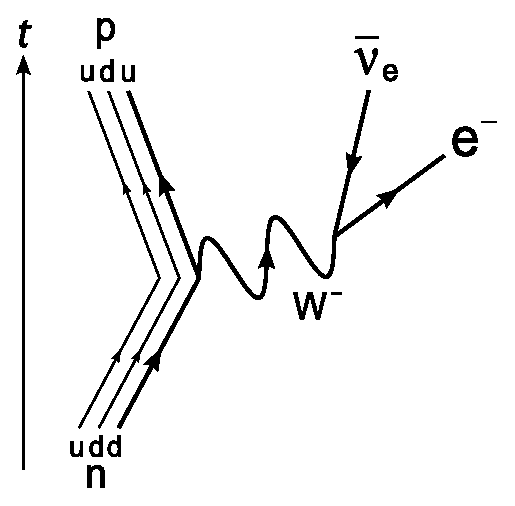
\includegraphics{assets/Beta_Negative_Decay.eps}
\caption{Feynman diagram of beta decay. The charged current weak interaction boson in this case is a $W^-$. Credit: Joel Holdsworth, within public domain.}
\label{fig:Beta_Negative_Decay}
\end{figure}

More generally, positron emission and electron capture are also neutrino related nuclear reactions which is explained in table \ref{table:Neutrino_Reactions}. In the context of astrophysics, (anti-)neutrinos also participate in nuclear reaction chains in stars, synthesis of heavy and rare elements and more.


\begin{table}[ht]
\centering
 \begin{tabular}{|c | c | c|} 
 \hline
 Reaction & Equation & Boson   \\ [0.5ex] 
 \hline
 Electron emission & ${}^A_Z X \to {}^A_{Z+1}X + e^- +\bar \nu_e$ & $W$  \\ 
 Positron emission & ${}^A_Z X \to {}^A_{Z-1}X + e^+ + \nu_e$ & $W$  \\
 Electron capture & ${}^A_Z X + e^- \to {}^A_{Z-1}X  + \nu_e$ &  $W$ \\
 Positron capture & ${}^A_Z X + e^+ \to {}^A_{Z+1}X  + \bar\nu_e$ &  $W$ \\
 [0.5ex] 
 \hline

 Electron annihilation &  $e^- + e^+  \to \nu_e + \bar\nu_e $  & $W$ \\
 Electron annihilation &  $e^- + e^+  \to \nu + \bar\nu $  & $Z$ \\
 [0.5ex] 
 \hline

  Neutrino capture & ${}^A_{Z}X + \overset{(-)}{\nu_e} \to {}^A_{Z\mp 1}X + e^\pm $ & W\\
  [1ex] 
 \hline
 $e^-\nu$ scattering & $e^- + \overset{(-)}{\nu_e} \to e^- + \overset{(-)}{\nu_e} $ &  $W$ \\
 $e^-\nu$ scattering & $e^{\pm} + \overset{(-)}{\nu_e} \to e^{\pm} + \overset{(-)}{\nu_e} $ &  $Z$ \\
 Neutrino scattering & $ {}^A_Z X + \overset{(-)}{\nu} \to {}^A_Z X + \overset{(-)}{\nu} $ &  Z\\
 [0.5ex] 
 \hline
 \end{tabular}
 \caption{Neutrino related nuclear or leptonic reactions}
\label{table:Neutrino_Reactions}
\end{table}

Astrophysical neutrino sources such as cores of stars, AGN, Gamma-ray bursts, and supernovae, reveals a lot of information about the sources. Though neutrinos are are weakly interacting particles thus rendering them hard to detect, it is an important subject to theoretically inspect neutrino productions in astrophysical processes.

One of the neutrino factories is the stellar core. Numerous nuclear reactions as well thermal neutrino production produce high number density neutrinos emissions. In this section, the nuclear reactions in stars are reviewed as well as the neutrino oscillation in the stars.



\subsection{Nuclear Reactions in Stars and Neutrino Flux}

pp chain and CNO cycle are the most important nuclear reactions in a star. Through different stages of its life, a star experience different nuclear reactions. Figure \ref{fig:pp_Chain_Branching} shows the dominant energy source of solar mass stars. In order to calculate the neutrino spectrum we need the neutrino production rate in each reaction and the branching ratios. The processes that emits neutrinos are the red reactions in Fig \ref{fig:pp_Chain_Branching}, which explicitly are

\begin{align}
&\mathrm{p+p\to {}^2H + e^+ +\nu_e},  & \mathrm{\leq 0.422MeV}\\
&\mathrm{{}^7Be + e^- \to {}^7Li + \nu_e} , &\text{0.862MeV for 90\%}\\
&&\qquad \text{0.384MeV for 10\%} \\
&\mathrm{{}^8B \to {}^8Be^* +e^+ +\nu_e},  & \mathrm{\leq 15 MeV}
\end{align}




\begin {figure*}%[!hbtp]
\centering
\begin{adjustbox}{width=\textwidth}
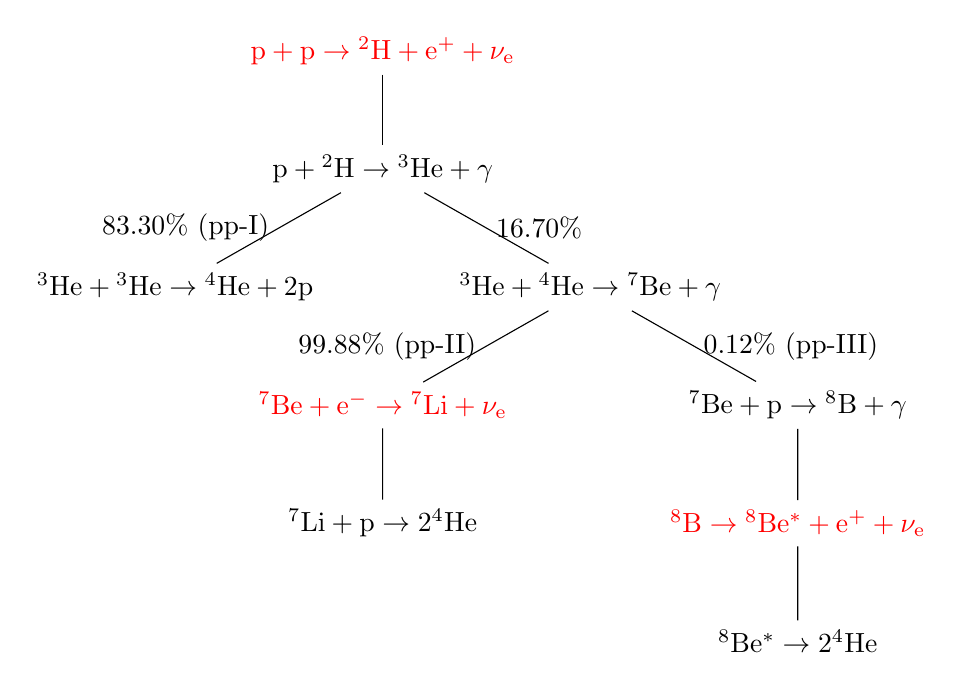
\begin{tikzpicture}[sibling distance=15em,
  every node/.style = {shape=rectangle,
    draw, align=center}
  edge from parent/.style = {draw, -latex},]]
  \node {\color{red}$\mathrm{p+p\to {}^2H + e^+ +\nu_e}$ }
    child { node {$\mathrm{p+{}^2H \to {}^3He + \gamma}$}
      child { node {$\mathrm{{}^3He+{}^3He \to {}^4 He + 2p }$}
          edge from parent node [left] {83.30\% (pp-I) } }
      child { node {$\mathrm{{}^3He+{}^4He \to {}^7 Be + \gamma }$}
        child { node { 
\color{red}$\mathrm{{}^7Be + e^- \to {}^7Li + \nu_e}$  
        }
        child { node { $\mathrm{{}^7Li + p \to 2{}^4He }$} }
        edge from parent node [left] {99.88\% (pp-II) } }
        child { node { $\mathrm{{}^7 Be + p \to {}^8 B + \gamma}$}
        child { node { \color{red}$\mathrm{{}^8B \to {}^8Be^* +e^+ +\nu_e}$ }
		child { node { $\mathrm{{}^8Be^* \to 2 {}^4He }$ } }}
        edge from parent node [right] {0.12\% (pp-III) } }
        edge from parent node [right] {16.70\%  } }};
\end{tikzpicture}
\end{adjustbox}
\caption{ pp chain with branching ratio\cite{Altmann2001} }
\label{fig:pp_Chain_Branching}
\end{figure*}


\begin{figure}[!hbtp]
\centering
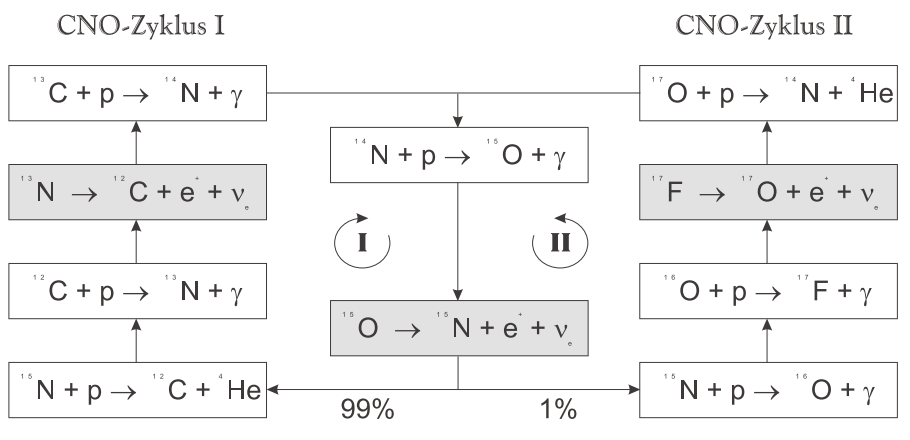
\includegraphics[width=\columnwidth]{assets/cno_cycle.png}
\caption{CNO cycle illustration.\cite{Adelberger2011a}}
\label{fig:cno_cycle}
\end{figure}


Solar neutrinos are mostly produced in pp reaction, Be electron capture and B decay, which are called pp neutrinos, Be neutrinos and B neutrinos. Even without knowledge of the detailed reactions, the conservation of lepton numbers will lead to the overall neutrino production

\begin{equation}
\mathrm{4p+2e^- \to {}^4He + 2\nu_e },
\end{equation}

where it is important to notice that two neutrinos are produced in each reaction. This overall reaction can either be pp chain or CNO cycle.

Using this simple relation, we can estimate the neutrino flux emitted by our sun. Given the kinetic energy produced in each reaction is the difference between the initial masses and the final masses, $Q_{pp}=4m_p+2m_e-m_{He4}=26.7\mathrm{MeV}$ where the mass of neutrinos are neglected since they are small compared with every other particle. On average, each neutrino carries away $0.2\mathrm{MeV}$ energy and the rest will be mostly in the form of thermal energy $Q_\gamma=26.3\mathrm{MeV}$. Number flux of thermal photons near Earth can be calculated using the solar constant $S_0$,

\begin{equation}
\Phi_\gamma = \frac{S_0}{Q_\gamma}.
\end{equation}

Since we know each reaction produces 2 neutrinos while producing $Q_\gamma$, which means that the number flux of neutrinos near Earth is roughly twice of the number flux of photons, i.e.,

\begin{equation}
\Phi_\nu = 2 \Phi_\gamma \approx 6\times 10^{10} \mathrm{cm^{-2}s^{-1}}.
\end{equation}


For such a large flux, understanding the role in stellar nuclear reaction and spectra is important.




\begin{figure}[!hbtp]
\centering
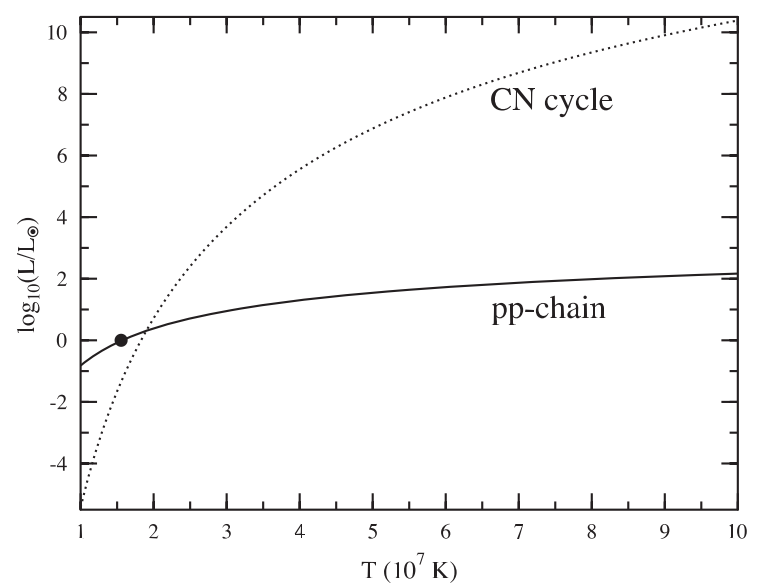
\includegraphics[width=\columnwidth]{assets/pp_chain_vs_cno.png}
\caption{The contribution to the luminosity by pp chain and CNO cycle as a function of temperature.\cite{Adelberger2011a} The black dot is at the solar core temperature.}
\label{fig:pp_chain_vs_cno}
\end{figure}












\subsection{Neutrino Oscillation}


Neutrinos are special particles that their flavor eigenstates are not the propagation eigenstates, which leads to neutrino flavor oscillations. Since neutrinos with different flavor interact with matter with different cross section, we need to investigate the neutrino flavor carefully. Even though only electron flavor neutrinos are produced, what we detect on Earth is different in flavor, which depends on two phenomena, neutrino vacuum oscillation and Mikheyev–Smirnov–Wolfenstein effect.

\subsubsection{Vacuum Oscillation}

To understand the neutrino vacuum oscillation phenomenon, we use two flavor neutrino as an example. In vacuum, propagation states are mass eigenstates, which is different from flavor eigenstates. The wave function in flavor eigenstates basis is related to wave function in mass eigenstates through an unitary matrix $\mathbf U$,

\begin{equation}
\Psi_f = \mathbb{U}_{\alpha i}\Psi_{v},
\end{equation}

where $\Psi_f$ is wave function in flavor basis and $\Psi_v$ is the wave function in vacuum mass eigenstate basis. The rotation matrix is

\begin{equation}
U = \begin{pmatrix} \cos\theta_v & \sin \theta_v \\ -\sin \theta_v & \cos \theta_v \end{pmatrix}.
\end{equation}

In vacuum basis, the Hamiltonian is free propagation, which is given by

\begin{equation}
H_v^{(v)} = \begin{pmatrix} E_1 & 0 \\
0 & E_2
\end{pmatrix},
\end{equation}

where

\begin{align}
E_i^{(v)} & = \sqrt{m_i^2 + p_i^2 } \\
& = p_i \sqrt{\frac{m_i^2}{p_i^2} + 1} \\
& \approx p_i + \frac{1}{2} \frac{m_i^2}{p_i}.
\end{align}

We assume the neutrinos have almost the same momentum, which is true since their mass is small, i.e., $p_i \approx E$. To first order, the Hamiltonian becomes

\begin{align*}
H_v^{(v)} &= \frac{1}{2E} \begin{pmatrix}
m_1^2 & 0 \\
0 & m_2^2
\end{pmatrix} + p \mathbb{I}\\
& =  \frac{1}{4E} \begin{pmatrix}
m_1^2 - m_2^2 & 0 \\
0 & m_2^2 - m_1^2
\end{pmatrix} \\
&\phantom{=}+ \frac{m_2^2 + m_1^2}{4E} \begin{pmatrix}
1 & 0 \\
0 & 1
\end{pmatrix} + \mathbf{I},
\end{align*}

where the identity matrices only give us an overall phase so we drop them. With the definition that $\Delta m^2 = m_2^2 - m_1^2$ The vacuum Hamiltonian in vacuum basis is simplify

\begin{equation}
H_v^{(v)} =  \frac{\Delta m^2}{4E} \begin{pmatrix}
-1 & 0 \\
0 & 1
\end{pmatrix},
\end{equation}

which leads to the simple solution for the wave function in vacuum basis

\begin{equation}
\Psi_v(t)^{(v)} = \begin{pmatrix}
c_1(0) e^{i\Delta m^2 t } \\
c_2(0) e^{ -i\Delta m^2 t } 
\end{pmatrix},
\end{equation}

where the initial condition is

\begin{equation}
\Psi_v(0)^{(v)} = \begin{pmatrix}
c_1(0) \\
c_2(0) 
\end{pmatrix}.
\end{equation}

In flavor basis, the wave function at anytime is

\begin{align}
\Psi_f(t) &= \mathbf{U}\Psi_v(t) \\
& = \begin{pmatrix} \cos\theta_v & \sin \theta_v \\ -\sin \theta_v & \cos \theta_v \end{pmatrix} \begin{pmatrix} c_1(0) e^{i\Delta m^2 t } \\
c_2(0) e^{ -i\Delta m^2 t }    \end{pmatrix} .
\end{align}

As seen in the nuclear reactions in the solar core, electron neutrinos are most abundant flavor. Initial condition is assumed to be electron flavor in the calculation which leads to the survival probability of electron flavor

\begin{equation}
P(\nu_e,t) = \Psi_f(0)^\dagger \Psi_f(t) = 1-\sin^2(2\theta_v)\sin^2\left( \frac{\Delta m^2 t}{4E} \right).
\end{equation}

Since neutrinos travel with velocity approximately the speed of light, we use $L = t$ where $L$ is the distance travelled. The survival probability is

\begin{equation}
P(\nu_e,L) =  1-\sin^2(2\theta_v)\sin^2\left( \frac{\Delta m^2 L}{4E} \right).
\end{equation}


The important parameter is the oscillation length of the neutrino flavor conversion. Here we have the oscillation frequency $\omega = \frac{\Delta m^2}{2E}$.

(Need a figure about the oscillation lengh here.)



\subsubsection{Mikheyev–Smirnov–Wolfenstein Effect}

The nature of neutrino oscillation means that flavor conversion occurs as long as their propagation eigenstates are not flavor eigenstates. We expect neutrino propagation eigenstates in matter are different from flavor states in general.\cite{wolf78} Using the fact that neutral current interactions between different flavor neutrinos and matter is independent of flavor, we only include the charged current, which will produce a effective potential for electron flavor. In flavor basis, the effective potential is

\begin{equation}
V=\frac{\sqrt{2}G_F n_e}{2} \sigma_3,
\end{equation}

where $G_F$ is Fermi constant, $n_e$ is number density of electrons. We also removed the identity in this matrix since it doesn't change our survival probability. The Hamiltonian with matter effect is the combination of vacuum oscillation and matter effect, which is, in flavor basis, explicitly,

\begin{equation}
H_m = \frac{ \Delta m^2 }{2E}\frac{1}{2}\begin{pmatrix} -\cos 2\theta_v & \sin 2 \theta_v \\ \sin 2\theta_v & \cos 2\theta_v  \end{pmatrix} + \frac{\sqrt{2}G_F n_e}{2} \sigma_3,
\end{equation}

where we used the result of flavor basis vacuum oscillation Hamiltonian

\begin{align}
H_v^{(f)}& = \mathbf{U} H_v^{(v)}\mathbf{U^\dagger} \\
&= \frac{ \Delta m^2 }{2E}\frac{1}{2}\begin{pmatrix} -\cos 2\theta_v & \sin 2 \theta_v \\ \sin 2\theta_v & \cos 2\theta_v  \end{pmatrix}.
\end{align}

Applying Pauli matrices and $\lambda = \frac{\sqrt{2}G_F n_e}{2}$ to this total Hamiltonian, it is rewritten as

\begin{equation}
H_m = \left(\frac{\lambda}{2} -\frac{ \omega }{2} \cos 2\theta_v \right) \boldsymbol{\sigma}_3  + \frac{ \omega }{2} \sin 2\theta_v \boldsymbol{\sigma}_1.
\end{equation}

Due to the off-diagonal terms in the Hamiltonian, the system will experience oscillations in flavor. A resonance, i.e., maximum mixing, dominates the system when the diagonal terms becomes zero,

\begin{equation}
\frac{\lambda}{2} -\frac{ \omega }{2} \cos 2\theta_v  = 0,
\end{equation}

which gives us the MSW resonance condition.

The importance of matter effect to our understanding of solar neutrinos is that it modifies the oscillation, which depends on the matter profile. For a solar mass star, we have almost adiabatic evolution of the neutrinos, which means that the instantaneous eigenstates and eigenvectors of Hamiltonian is good enough for the time dependent Schr\"{o}dinger equation. 


For simplicity, we define the vacuum frequency and the hatted quantities

\begin{align}
\omega &= \frac{\Delta m^2}{2E} \\
\hat\lambda & = \frac{\lambda}{\omega}.
\end{align}

The eigenstates, derived by diagonalizing the Hamiltonian, are

\begin{align}
E_1 &= \frac{\omega}{2}\sqrt{ \hat\lambda +1 -  2\hat\lambda \cos 2\theta_v }\\
E_2 &= -\frac{\omega}{2}\sqrt{ \hat\lambda +1 -  2\hat\lambda \cos 2\theta_v }.
\end{align}


\begin{figure}
\centering
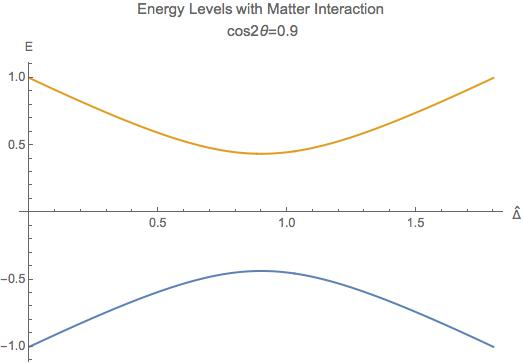
\includegraphics[width=\columnwidth]{assets/mswEnergyLevels.jpg}
\caption{The two energy levels in matter effect. The energy has unit $\omega/2$ while the potential has unit $\omega$.}
\label{fig:mswEnergyLevels}
\end{figure}

Figure \ref{fig:mswEnergyLevels} shows the two energy levels. For very high matter density, which interact with electron neutrinos more through charged current, electron flavor is composed almost with heavy propagation eigenstate. However, as the matter density becomes lower, the heavy propagation state will be gradually transformed to the other flavors since electron flavor in vacuum is composed mostly the light mass state.

In summary, even though only electron flavor neutrinos are produced in the core of a solar mass star, the neutrino flavor will be converted to the other flavors due to matter interaction.









\section{Neutrino Energy}







\begin{figure}[!hbtp]
\centering
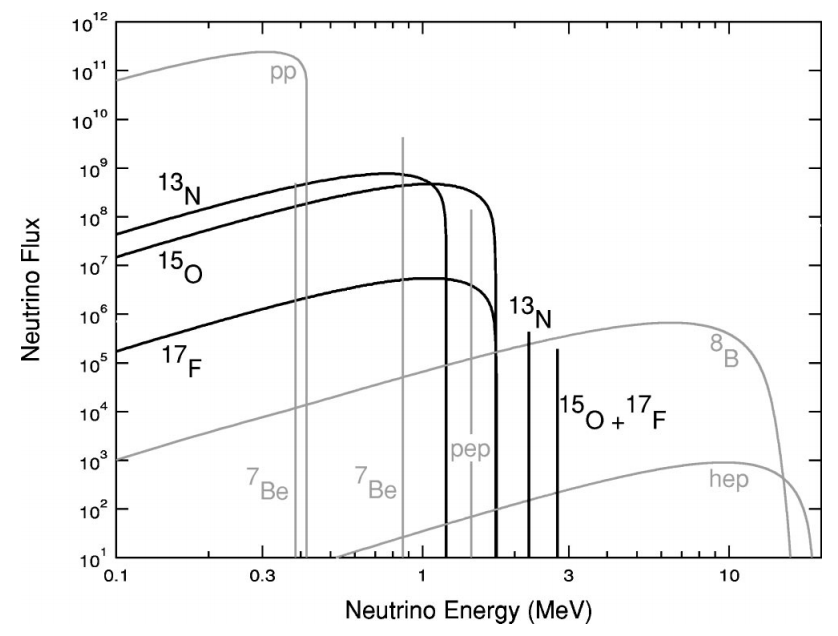
\includegraphics[width=\columnwidth]{assets/neutrino_spectra.png}
\caption{Neutrino spectra of the four pp chain and CNO cycle. Units are $\mathrm{cm^{-2} s^{-1} MeV^{-1}}$ for flux and $\mathrm{MeV}$ for neutrino energy.\cite{Stonehill2004}}
\label{fig:neutrino_spectra}
\end{figure}









%%%%%%%%%%%%%%%%%%%%%%%%%%%%%%%%%%%%%%%%%%%%%%%%%%%%%%%%%%%%%%

\medskip

%Sets the bibliography style to UNSRT and imports the 
%bibliography file "samples.bib".
%\bibliographystyle{unsrt}
\bibliography{ref}




\end{document}
%
% ****** End of file aipsamp.tex ******
